\section{碳的化学性质}\label{sec:3-3}

碳的各种同素异形体都有同样的化学性质。在常温下,碳的化学性质不活泼。
碳受日光照射或跟空气、水分接触,不容易起变化。碳也不跟一般的氧化剂起反应。
我国古代的字画,虽年深日久仍不变色,就是由于用墨书写或绘制的缘故。
随着温度的升高,碳的活动性大大增强。在高温下,碳能跟多种物质起反应。

\subsection{碳跟氧气和非金属的反应}

碳在氧气或空气里充分燃烧,生成二氧化碳,同时放出大量的热。
\begin{fangchengshi}
    \ce{ C + O2 = CO2 }
\end{fangchengshi}

当碳燃烧不充分的时候,就生成一氧化碳,同时放出热。
\begin{fangchengshi}
    \ce{ 2C + O2 = 2 CO }
\end{fangchengshi}

碳在高温下能跟多种非金属化合。把木炭灼烧,然后通入硫的蒸气,就生成二硫化碳的蒸气。
\begin{fangchengshi}
    \ce{ C + 2S $\xlongequal{\text{高温}}$ $\underset{\text{二硫化碳}}{\ce{CS2}}$ }
\end{fangchengshi}

纯净的二硫化碳是一种易挥发的无色液体。


\subsection{碳跟某些氧化物的反应}

碳的一个重要的化学性质是还原性,它能在较高温度下夺取某些含氧化合物里的氧,使其它元素还原。
例如,炽热的碳能使二氧化碳还原成一氧化碳。
\begin{fangchengshi}
    \ce{ CO2 + C $\xlongequal{\Delta}$ 2CO }
\end{fangchengshi}

跟碳在氧气里燃烧时放出热量的反应不同,上面的碳跟二氧化碳的反应不但没有放出热,而且还吸收热。
化学上把放出热的化学反应叫做\zhongdian{放热反应},吸收热的反应叫做\zhongdian{吸热反应}。
所以碳在氧气里燃烧所起的反应是放热反应,碳使二氧化碳还原的反应是吸热反应。

\begin{wrapfigure}[10]{r}{5cm}
    \centering
    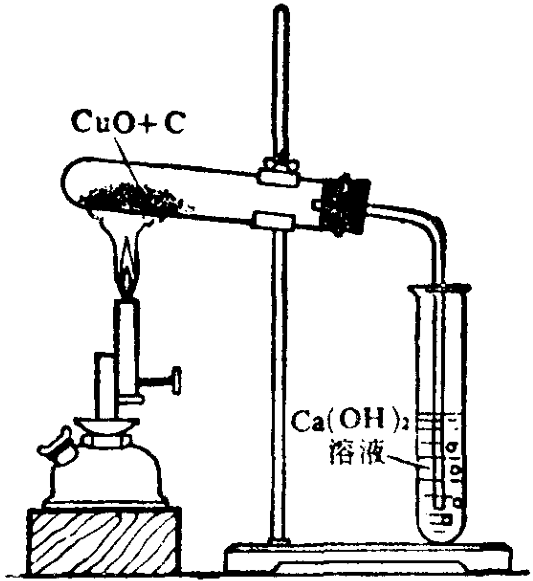
\includegraphics[width=4cm]{../pic/czhx1-ch3-4}
    \caption{用木炭还原氧化铜}\label{fig:3-4}
\end{wrapfigure}

\wrapfiguretrick

\begin{shiyan}
    把黑色氧化铜和木炭粉的混和物放入固定在架台上的试管里,
    试管口装有通入澄漪的石灰水的导管(图\ref{fig:3-4}),
    用酒精喷灯或煤气灯给试管加热几分钟,观察石灰水发生的变化。
    把试管里的粉末倒在纸上,仔细观察这些粉末。
\end{shiyan}

石灰水变成浑浊,为什么?从倒在纸上的粉末里可以看到什么?为什么?

倒在纸上的粉末里可以看到红色的铜,这因为在加热的时候,木炭能从氧化铜里还原出铜来。
\begin{fangchengshi}
    \ce{ 2CuO + C $\xlongequal{\text{高温}}$ 2Cu + CO2 ^ }
\end{fangchengshi}

因此,碳是还原剂,氧化铜是氧化剂。

在工业生产里,当加热到 1000 ℃ 以上时,焦炭可以将铁和锌从它们的氧化物矿石里还原出来。


\begin{xiti}

\xiaoti{比较碳和氢气的化学性质。}


\xiaoti{写出碳跟下列物质起反应的化学方程式,其中(2)、(3)要求指出氧化剂和还原剂。 \\
    (1) 氧气, (2) 氧化铜, (3) 氧化锌。
}

\xiaoti{在埋木料或木柱之前,为什么有时要把埋入地里的一段的表面用火微微烧焦?}

\xiaoti{碳在高温时还原三氧化二铁的化学方程式是:
    \begin{fangchengshi}
        \ce{ 2Fe2O3 + 3C $\xlongequal{\text{高温}}$ 4Fe + 3CO2 ^ }
    \end{fangchengshi}
    要使  50 克三氧化二铁完全还原,至少需碳多少克?
}

\end{xiti}

